\section{Computazione}
Finalmente vediamo come opera una MdT su qualche problema di
esempio. La \textbf{configurazione corrente} di una MdT viene
identificata $(q, u, \sigma, v)$ dove
\begin{itemize}
	\item $q$ è lo stato corrente.
	\item $u$ è la stringa a sinistra del carattere attuale.
	\item $\sigma$ è il carattere attuale.
	\item $v$ è il resto della stringa che termina con un
	      carattere non nullo.
\end{itemize}
La situazione corrente di una MdT può essere espressa più
comodamente con $(q, u \underline{\sigma} v)$. Graficamente
una MdT appare in questo modo
\begin{center}
	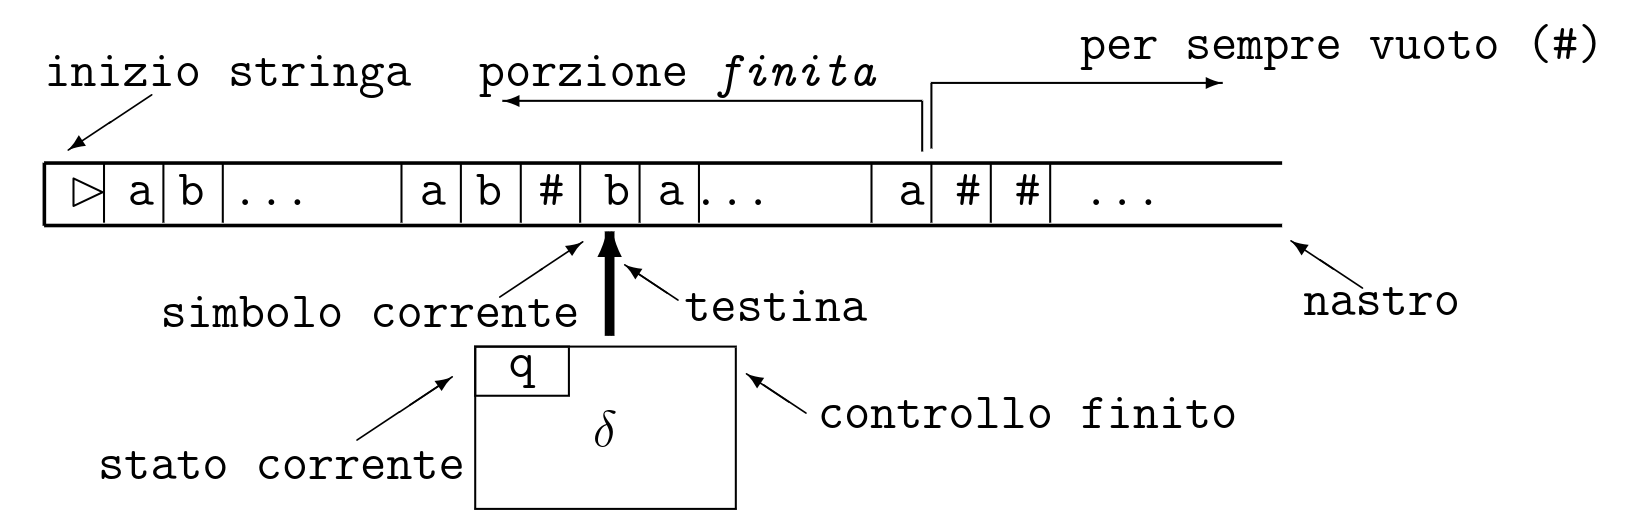
\includegraphics[scale=0.225]{images/turing.png}
\end{center}
Tenendo a mente questa figura possiamo provare a costruire la
nostra prima MdT.

\begin{example} \label{ex: 11}
	Vogliamo costruire una MdT in grado di dirci se la stringa
	binaria in input contiene una sottosequenza composta da
	due $1$ consecutivi.

	Per costruire la nostra macchina abbiamo bisogno di due
	stati ($q_0$ e $q_1$), di due simboli ($0$ e $1$) e di
	una funzione di transizione $\delta$.

	Per capire se la stringa in input contiene almeno una
	sottostringa composta da due $1$ consecutivi, iniziamo
	con lo stato iniziale $q_0$, il quale indica sia lo stato
	inziale della macchina sia lo stato in cui la macchina
	deve transire ogni qual volta incontra uno $0$.

	Abbiamo poi bisogno di uno stato $q_1$ in cui la macchina
	transisce quando incontra un $1$ nella sequenza dopo essere
	stata in uno stato $q_0$.

	Se ci troviamo nello stato $q_1$ e incontriamo un altro $1$
	la macchina transisce nello stato $h$ di terminazione. La
	funzione $\delta$ di transizione che deriva dai seguenti
	ragionamenti è la seguente
	\begin{center}
		\begin{tabular}{|c|c|c|}
			\hline
			$q$   & $\sigma$ & $\delta(q, \sigma)$ \\
			\hline
			$q_0$ & $\start$ & $q_0, \start, R$    \\
			$q_0$ & $0$      & $q_0, \#, R$        \\
			$q_0$ & $1$      & $q_1, \#, R$        \\
			$q_1$ & $0$      & $q_0, \#, R$        \\
			$q_1$ & $1$      & $h, \#, -$          \\
			\hline
		\end{tabular}
	\end{center}
	Come possiamo notare, ogni volta che incontriamo un
	carattere lo "cancelliamo" scrivendo $\#$ ma avremmo potuto
	lasciare il numero che incontravamo. Vediamo una possibile
	simulazione di esecuzione con la seguente stringa binaria
	in input
	\[ 01011 \]
	La nostra configurazione iniziale è
	\[ q_0 / \underline{\start} 01011 \]
	dove il simbolo sottolineato è quello su cui si trova il
	cursore. La sequenza di operazioni sarà quindi la seguente
	\begin{align*}
		q_0 / & \underline{\start} 01011       \\
		q_0 / & \start \underline{0} 1011      \\
		q_0 / & \start \# \underline{1} 011    \\
		q_1 / & \start \#\# \underline{0} 11   \\
		q_0 / & \start \#\#\# \underline{1} 1  \\
		q_1 / & \start \#\#\#\# \underline{1}  \\
		h /   & \start \#\#\#\# \underline{\#}
	\end{align*}
	Il calcolo è dunque terminato con successo.
\end{example}

Per vedere una MdT in azione è possibile visitare questo
\href{https://turingmachinesimulator.com/}{sito} in cui è
possibile programmare una MdT oppure eseguire esempi già
proposti.

\subsection{Configurazione e computazione}
Come abbiamo detto precedentemente, una \textbf{configurazione}
è definita dalla quadrupla
\[ \gamma = (q, u, \sigma, v) \]
Ciò che non abbiamo detto è che gli elementi di $\gamma$
appartengono al seguente insieme
\[
	\gamma \in (Q \cup \{ h \}) \times
	\Sigma^* \times \Sigma \times \Sigma^F
\]
L'ultimo insieme ($\Sigma^F$) è un po' particolare, è infatti
definito come
\[
	\Sigma^F = \Sigma^* \cdot \left( \Sigma \backslash
	\{ \# \} \right) \cup \{ \epsilon \}
\]
quindi possiamo scrivere la stringa $v$ come
$\sigma_0 \sigma_1 \dots \sigma_n$, con $\sigma_n \neq \#$,
al posto della stringa infinita composta dai vari $\sigma$ e
con infiniti $\#$ alla fine.

Si noti però che un qualsiasi carattere $\sigma_i$ con $i < n$
può essere $\#$ ed inoltre la stringa $u$ può essere vuota
solo quando il carattere corrente è $\start$. La convenzione
impone quindi di scrivere la configurazione iniziale del primo
esempio fatto, in questo modo
\[ (q_0, \start 01011, \epsilon) \]

\begin{definition}
	Una \textbf{computazione} è una successione finita di
	passi
	\[ (q_0, w) \to^* (q', w') \]
	dove $\to^*$ è la chiusura riflessiva e transitiva di
	$\to$. Ovviamente se vi sono $n$ passi, la computazione
	è lunga $n$ e dunque scriveremo $\to^n$.
\end{definition}

Definiamo meglio cos'è un \textbf{passo di computazione},
procedendo per casi e considerando $a$, $b$ e $c$ come elementi
generici di $\Sigma$.
\begin{itemize}
	\item $(q, u \underline{a} v) \to (q', u \underline{b} v)$
	      se $\delta (q, a) = (q', b, -)$.
	\item $(q, u c \underline{a} v) \to
		      (q', u \underline{c} b v)$
	      se $\delta (q, a) = (q', b, L)$.
	\item \begin{enumerate}
		      \item $(q, u \underline{a} c v) \to
			            (q', u b \underline{c} v)$
		            se $\delta (q, a) = (q', b, R)$.
		      \item $(q, u \underline{a}) \to
			            (q', u b \underline{\#})$
		            se $\delta (q, a) = (q', b, R)$.
	      \end{enumerate}
\end{itemize}
In questo modo garantiamo che ciascun passo abbia effetto
limitato sulle configurazioni, come richiesto dalla seconda
parte del punto 2 nell'\hyperref[sec: algoritmo]{idea intuitiva
	dell'algoritmo}.

Allo stesso modo possiamo immaginarci che se partiamo da uno
stato iniziale $(q_0, \underline{\start} w)$, dopo un certo
numero di passi arriviamo in uno stato $(q', w')$.

\begin{definition} \label{def: convergenza}
	Diciamo che una computazione \textbf{termina} o
	\textbf{converge} ($\downarrow$) se e solo se lo stato
	finale è $h$. Nell'esempio \ref{ex: 11} fatto qui sopra
	$q' = h$.

	Diciamo invece che la computazione \textbf{non termina}
	o \textbf{diverge} ($\uparrow$) se e solo se per ogni
	$q'$ e $w'$ tali che
	\[ (q_0, w) \to^* (q', w') \]
	esistono $q''$ e $w''$ tali che
	\[ (q', w') \to^* (q'', w'') \]
	ovvero tali che è sempre possibile fare un nuovo passo di
	computazione.
\end{definition}

Come possiamo vedere, le MdT definite in questo modo,
rispettano l'idea intuitiva di algoritmo che abbiamo dato
all'inizio.

\begin{example} \label{ex: non termina}
	Facciamo un esempio di computazione che non termina mai
	tramite una macchine che semplicemente non contiene il
	simbolo $h$ di terminazione.
	\begin{center}
		\begin{tabular}{|c|c|c|}
			\hline
			$q$   & $\sigma$ & $\delta$             \\
			\hline
			$q_0$ & $\start$ & $q_0$, $\start$, $R$ \\
			$q_0$ & $a$      & $q_0$, $a$, $R$      \\
			$q_0$ & $\#$     & $q_0$, $\#$, $R$     \\
			\hline
		\end{tabular}
	\end{center}
\end{example}

Proviamo ora a fare un esempio più concreto di una MdT che
calcola qualcosa di più sensato rispetto agli esempi visti
fino ad ora.

\begin{example}
	Questa MdT si propone di calcolare la somma di due numeri
	$n$ ed $m$, dove $n$ ed $m$ sono rappresentati in notazione
	unaria tramite il simbolo $|$ ripetuto $n$ (o $m$) volte.
	La funzione $\delta$ è definita dalla seguente tabella
	\begin{center}
		\begin{tabular}{|c|c|c|}
			\hline
			$q$   & $\sigma$ & $\delta$         \\
			\hline
			$q_0$ & $\start$ & $q_0, \start, R$ \\
			$q_0$ & $|$      & $q_0, |, R$      \\
			$q_0$ & $+$      & $q_1, |, R$      \\
			$q_1$ & $|$      & $q_1, |, R$      \\
			$q_1$ & $\#$     & $q_2, \#, L$     \\
			$q_2$ & $|$      & $h, \#, -$       \\
			\hline
		\end{tabular}
	\end{center}
	Il simbolo $+$ deve essere tra le due sequenze di $|$.
	Proviamo ora ad eseguire la computazione per il calcolo
	di $1 + 2$, partendo dalla configurazione iniziale
	\[ q_0/ \quad \underline{|} + | | \]
	Svolgiamo quindi i seguenti passi
	\begin{gather*}
		(q_0, \; \underline{\start} | + | | ) \to
		(q_0, \; \start \underline{|} + | | ) \\
		(q_0, \; \start \underline{|} + | | ) \to
		(q_0, \; \start | \underline{+} | | ) \\
		(q_0, \; \start | \underline{+} | | ) \to
		(q_1, \; \start | | \underline{|} | ) \\
		(q_1, \; \start | | \underline{|} | ) \to
		(q_1, \; \start | | | \underline{|} ) \\
		(q_1, \; \start | | | \underline{|} ) \to
		(q_1, \; \start | | | | \underline{\#} ) \\
		(q_1, \; \start | | | | \underline{\#} ) \to
		(q_2, \; \start | | | \underline{|} \# ) \\
		(q_2, \; \start | | | \underline{|} \# ) \to
		(h, \; \start | | | \underline{\#} \# )
	\end{gather*}
	per concludere che il calcolo termina dato che siamo
	giunti nello stato speciale $h$. Come possiamo vedere il
	nostro risultato è dato dal numero di $|$ rimanente.
\end{example}

Un altro tipico esempio di utilizzo di queste macchine è
quello di decidere se una stringa è palindroma. In questo
caso descriviamo brevemente quale sarebbe l'idea.
\begin{enumerate}
	\item Si controlla il primo carattere della stringa, lo si
	      sovrascrive con $\start$ e si passa in uno stato
	      specifico per quel carattere (supponendo che il primo
	      carattere sia $a$, si passa in $q_a$).
	\item Si arriva in fondo alla stringa e si controlla che
	      l'ultimo carattere sia uguale al primo, se sì, lo
	      si sovrascrive con un $\#$.
	\item Si torna indietro fino al primo $\start$ che si
	      incontra.
\end{enumerate}
Si ripete il procedimento finché non si esaurisce tutta la
stringa o finché non fallisce.